% !TeX root = ../main.tex
% Add the above to each chapter to make compiling the PDF easier in some editors.

\chapter{Implementation}\label{chapter:implementation}

As explained in \autoref{sec:terminology}, from now on the term Firmware ID (FWID) will be used instead of the previously used term TCB Component Identifier (TCI).

\section{Overview}


We run our implementation on ARM's Fixed Virtual Platform~(FVP)\footnote{\url{https://developer.arm.com/Tools\%20and\%20Software/Fixed\%20Virtual\%20Platforms}} which is a complete simulation of the Armv8-A architecture including TrustZone.

To do this, we use the software infrastructure provided by OP-TEE for various platforms, including FVP\@.
OP-TEE uses the TrustedFirmware-A~(TF-A)\footnote{\url{https://www.trustedfirmware.org/projects/tf-a/}} package from ARM as firmware boot components.
However, we mock their attestation, i.e., their Alias certificates are statically compiled into the binaries instead of being dynamically generated, as TF-A does not implement DICE\@.
The development efforts to implement that exceeds the benefits, as the concept can also be demonstrated with mocked certificates.
For that, only the certificates up to the OP-TEE~OS are mocked, including OP-TEE~OS's private key to sign the subsequent Alias certificate, which is our EKcert.

Our implementation with compilation and running instructions can be found on GitHub\footnote{\url{https://github.com/akorb/master-thesis-meta}}.

\section{Boot chain}

The boot process is depicted in \autoref{fig:boot_chain}.
DICE is the root of trust, because incorrect behavior remains undetected and would jeopardize the security of our attestation process.

\begin{figure}[htpb]
  \centering
  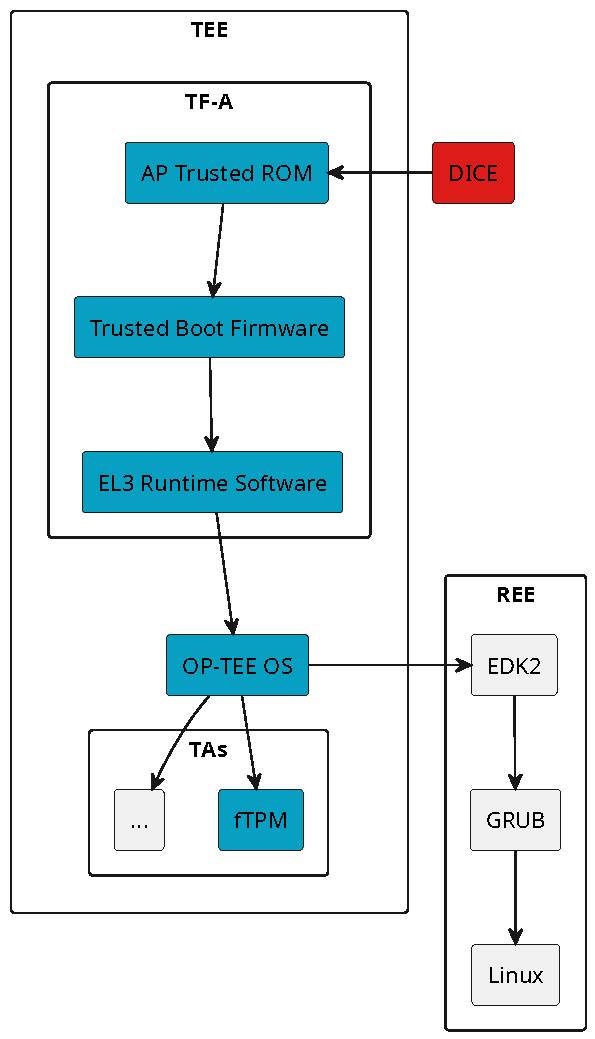
\includegraphics[width=0.8\linewidth]{figures/boot-chain.pdf}
  \caption{The boot chain of our system running in Arm's FVP\@. Blue: Represented by our yielding certificate chain. Red: Root of trust for verifier, and assumed to be present.}\label{fig:boot_chain}
\end{figure}



\paragraph{DICE}
Theoretically, the boot chain begins with the DICE hardware, but this is not included in FVP\@.
Therefore, we simply assume its presence by mocking the first few certificates of the yielding certificate chain.
Furthermore, it is independent hardware, and therefore, neither part of the TEE nor the REE\@.

\paragraph{TF-A}
After reset, the CPU executes within the secure world.
That is also the reason why machines that are unaware of the separation between secure world and normal world are running in the secure world, as they never modify the execution environment of the processor.
This also ensures that TrustZone unaware systems have all expected privileges, which would be restricted in the normal world.
The Application Processor~(AP) Trusted ROM sets up the platform-specific exception vectors.
The Trusted Boot Firmware enables the MMU, performs the platform security setup, and other tasks.
The final component of TF-A --- EL3 Runtime Software --- replaces the simple and rudimentary initialization performed by the AP Trusted ROM with more complete configurations by detecting the system topology, and enabling normal world software to function correctly.
The EL3 Runtime Software also provides the monitor which conducts the context switches between the secure world and the normal world.
More complete and detailed information can be found in the TF-A documentation\footnote{\url{https://trustedfirmware-a.readthedocs.io/en/latest/design/firmware-design.html}}.

\paragraph{OP-TEE~OS}
Finally, the OP-TEE~OS\footnote{\url{https://github.com/OP-TEE/optee_os}} is loaded and executed.
Just like an ordinary operating system, it initializes its functions offered to the user space of the secure world, i.e., the trusted applications.

\paragraph{Trusted Applications}

Our TA in focus is the firmware TPM\footnote{\url{https://github.com/microsoft/ms-tpm-20-ref/}}\@.
It consists of the reference code by Microsoft which implements a TPM, and the stub code, which provides and implements the interfaces required to be a TA of OP-TEE\@.
This fTPM only allows a single connection at any time, i.e., it prohibits concurrent access as this could lead to inconsistent states.
This also mirrors hardware TPMs, which are usually attached via serial buses like SPI to the processor.
Typically, the only entity that communicates with the fTPM is a Linux kernel module\footnote{\url{https://docs.kernel.org/security/tpm/tpm_ftpm_tee.html}}, so it is transparent to the user applications whether the TPM is implemented in firmware or hardware.
Note that TAs are not started automatically.
In fact, we are not aware of any function provided by OP-TEE~OS to register a TA to be started during the boot process. 
Instead, TAs are initialized the first time someone wants to interact with them.

\paragraph{EDK2}
TianoCore EDK II\footnote{\url{https://github.com/tianocore/edk2}} is the first component launched in the normal world.
It is a reference implementation of UEFI~\cite{UEFI} by Intel.

\paragraph{GRUB}
The GNU GRand Unified Bootloader\footnote{\url{https://www.gnu.org/software/grub/}} is a bootloader which is responsible for loading and transferring control to OS kernel software.

\paragraph{Linux}
As expected, the final component to boot is the Linux\footnote{\url{https://www.kernel.org/}} operating system.

\section{Firmware TPM initialization}

Initialization begins with the derivation of all secrets from the CDI\@.
Note that we mocked the CDI that would be passed from OP-TEE OS to the fTPM in practice.
However, OP-TEE OS does not implement DICE\@.

We use the Mbed TLS library\footnote{\url{https://mbed-tls.readthedocs.io/en/latest/}} providing cryptographic primitives for the derivation of the secrets, and also to build X.509 certificates.
Mbed TLS is already part of OP-TEE, and its functionality is modular and allows certain functionality to be activated or deactivated at a fine granular level.
Since the target machines are embedded devices with limited resources, the user should only activate the functions that he really needs.
We therefore had to activate some functions.

The formulas which derive secrets directly from the CDI (\autoref{eq:storage_key_formula}, \autoref{eq:eps_formula}) use a keyed-hash message authentication code~(HMAC) function.
This is inspired by the CDI derivation proposed in the DICE hardware requirements specification~\cite{dice-hardware-reqs}.
Actually, it proposes two functions to combine information to a new secret.
A simple hash function, and the HMAC function.
It also states that it recommends the HMAC function which calculation takes a little more time, but protects the CDI with twice the level than the simple hash function.
% https://nvlpubs.nist.gov/nistpubs/SpecialPublications/NIST.SP.800-57pt1r5.pdf (Table 3) shows that the HMAC version has roughly double security strength
This is backed by Jäger et al.~\cite{Jaeger2017}, and NIST SP 800--57~\cite{Barker2020}.
We declare the inner hash function used by the HMAC according to the required data size of the secret.
For example, for storage encryption, we use AES-256, and therefore, use the SHA256 function to retrieve a key with a sufficient size.
The HMAC functions are seeded with a fixed character string that describes the purpose of the output secret, e.g., `EPS'.

% Formula from (2) in https://trustedcomputinggroup.org/wp-content/uploads/Hardware-Requirements-for-Device-Identifier-Composition-Engine-r78_For-Publication.pdf
\begin{align}
  \label{eq:storage_key_formula}
  K_{storage} &= HMAC_{SHA256}(CDI,\ `DATA\ STORAGE\ KEY\text{'})\\
  \label{eq:eps_formula}
  EPS &= HMAC_{SHA512}(CDI,\ `EPS\text{'})\\
  \label{eq:ek_formula}
  EK  &= KDF(EPS,\ EK_{template})
\end{align}

\begin{figure}[htb]
  \centering
  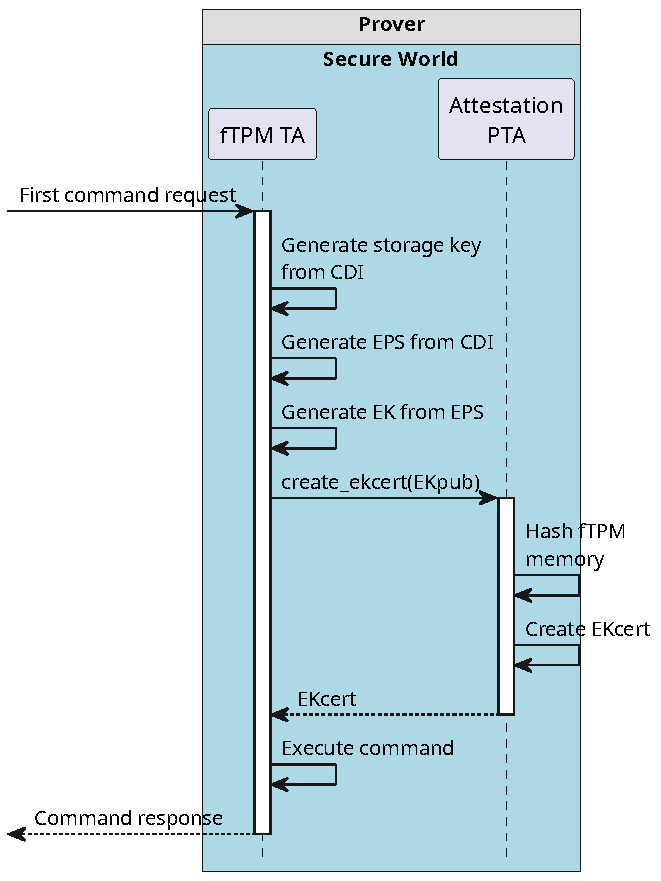
\includegraphics[width=0.62\linewidth]{figures/tpm-initialization.pdf}
  \caption{A UML sequence diagram describing the initialization of our firmware TPM\@.}\label{fig:ftpm_initialization}
\end{figure}


We must ensure we retrieve exactly the same EK as the TPM would generate by a \texttt{TPM2\_CreatePrimary} command with our EK template.
Therefore, we use the firmware TPM internal functions to generate the EK\@.
The EK consists of a private and a public portion.
The private part never leaves the TPM, and the public portion is forwarded to the attestation PTA to be used as the subject key for EKcert, as shown by \autoref{fig:ftpm_initialization}.
A pseudo trusted application~(PTA) provides the same interfaces as an ordinary TA, but is actually not a separate process in the user space of the secure world, but runs as part of the OP-TEE OS\@.
Therefore, it has more privileges than an ordinary TA\@.
These privileges are required by the attestation PTA provided by OP-TEE to read the memory of the calling TA, which is required for attestation.
The attestation PTA creates EKcert with EKpub as subject signed by OP-TEE's private key containing the FWID of the fTPM TA\@.
Note that fTPM has never access to private alias key of OP-TEE OS, so it cannot spoof its Alias Cert/EKcert.

The attestation PTA hashes the memory pages of the calling TA that are executable or read-only data, i.e., are constant.
It can also simply extract the hash embedded in the TA's binary header.
A TA is an ELF binary wrapped in an OP-TEE specific format, which header contains a signature over all metadata and the payload, i.e., the ELF executable.
While it is simpler and faster, it does not attest the TA's dynamically linked libraries.
Although the reference firmware TPM does not link dynamically to any library, we use the attestation of the memory data to be more future-proof.

To embed the FWID into the EKcert, we use the X.509 extension defined by the DICE Attestation Architecture~\cite{TCGAttestation2021}.
Therein, the TCB Info Evidence Extension is defined.
It allows many FWIDs to be embed into an X.509 certificate.
Our implementation always only stores one FWID into each Alias certificate or EKcert.
However, the privacy focused architecture explained in \autoref{sec:privacy} could leverage the possibility to store multiple FWIDs in the extension.
Each FWID consists of an identifier of the hash algorithm used, and the according digest.
We use SHA256.
The TCB Info Evidence Extension is defined formally in the ASN.1 description language.
Consequently, we use ASN1c\footnote{\url{https://github.com/vlm/asn1c}} to translate this formal definition to C~code.
In particular, we use a self-compiled version of ASN1c, since its last official release dates back to 2017, whereby its generated C~code throws various warnings with a modern C~compiler.

The resulting certificate generated by the attestation PTA is returned to the firmware TPM, which also has access to all preceding certificates.
In our implementation, these preceding certificates are simply mocked.

\section{Firmware TPM attestation}

\begin{figure}[htb]
  \centering
  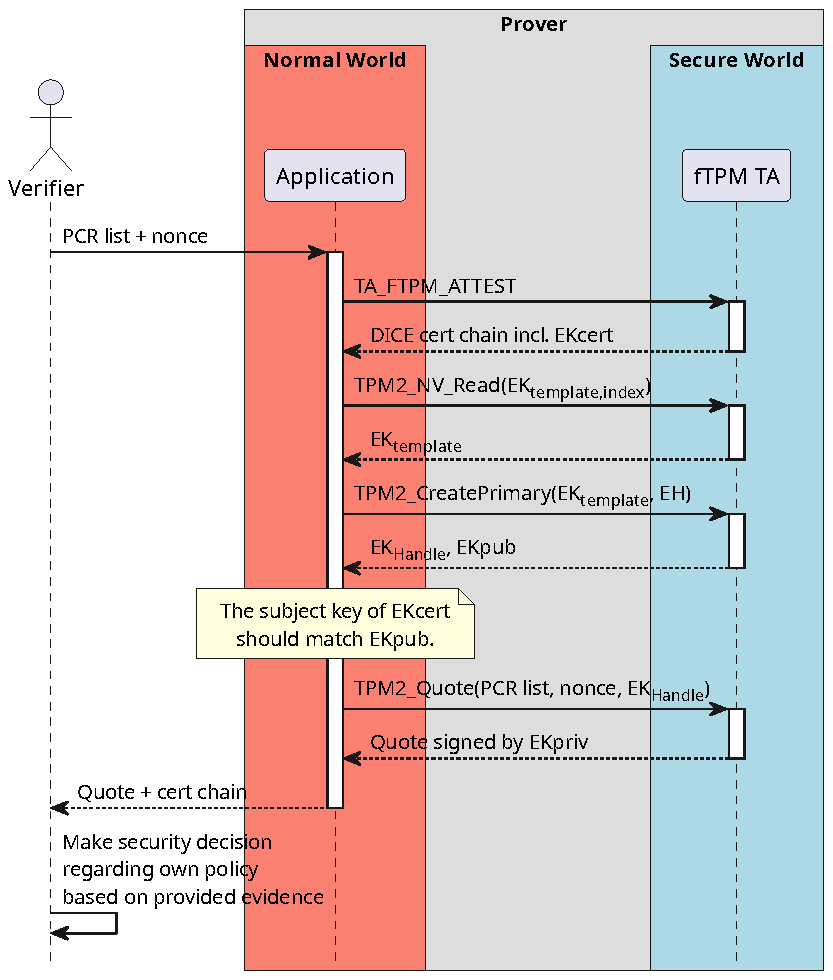
\includegraphics[width=0.74\linewidth]{figures/tpm-attestation.pdf}
  \caption{A UML sequence diagram describing the attestation of our firmware TPM\@.}\label{fig:ftpm_attestation}
\end{figure}


We added a new TA command called \texttt{TA\_FTPM\_ATTEST} to the firmware TPM to obtain the entire certificate chain from any application.
Normally, this command is issued by the application that performs the prover part of the remote attestation.
We would like to emphasize that we do not refer to a new TPM command that would imply an extension of the TPM specification, but a new TA command that is intercepted by the OP-TEE stub code of the fTPM and processed without the involvement of the TPM-specific core code.

Recall that we earlier described that the firmware TPM TA only ever allows a single connection to it, which is usually a Linux module that provide the \texttt{/dev/tpm0} and \texttt{/dev/tpmrm0} nodes to communicate with the fTPM\@.
We have therefore implemented the prover's side of the remote attestation with the ability to unload this Linux module before issuing \texttt{TA\_FTPM\_ATTEST}, and then load the Linux module again.

The prover's user space application starts with issuing the \texttt{TA\_FTPM\_ATTEST} command to the firmware TPM, as shown by \autoref{fig:ftpm_attestation}.
Consequently, it receives the certificate chain created by DICE with the EKcert as leaf certificate.

Afterwards, the prover wants the TPM to create the EK including its private portion.
For that, it first reads the EK template from the fTPM's non-volatile~(NV) storage.
We create the EK template within the firmware TPM in code on its first launch after any reset.
Thus, it is always present.
It is stored in the NV index \texttt{0x01c00004} as defined by the TPM specification for RSA 2048 EK templates~\cite{tcg-ek}.
We set the attributes for this NV index as defined by the TPM PC Client specification~\cite{tcgPcClient}. % 4.5.2.1
Thereby, the EK template in the NV can only be written or deleted if a specific policy is fulfilled.
However, the policy is empty, which can never be fulfilled.
This results in a non-deletable EK template.
We also store the EKcert in the NV index \texttt{0x01c00002} as defined by the TCG EK Credential Profile~\cite{tcg-ek} with the same attributes as the respective template.
The template and certificate do not contain any sensitive material and can hence be read by anyone using the command \texttt{TPM2\_NV\_Read}.

Consequently, it then sends the template that has just been retrieved back to the TPM as part of the command \texttt{TPM2\_CreatePrimary}.
Since this command creates a primary key, no parent has be specified as the primary seed of the specified hierarchy is used instead.
Of course, we specify the endorsement hierarchy (EH), which makes the TPM use the endorsement primary seed (EPS) derived from the CDI to generate the EK\@.
The TPM returns a handle to the EK just created, which is an integer, as well as the public part of the EK\@.
The private part of the EK is not returned, as this never leaves the TPM in plain text.

Eventually, the prover wants to create a quote to establish trust to the prover's system state in the normal world, and to prove that it is in control of the EKpriv.
So, it issues the command \texttt{tpm2\_quote} to the TPM, specifying the PCR registers requested by the verifier, the verifier supplied nonce, and the handle to the EK just generated.

The prover's application handling the remote attestation is now in possession of the certificate chain, and a quote.
It transmits both to the verifier.
The verifier extracts the EKpub which is the subject key of the EKcert.
With that, it can verify the digital signature of the quote.
The ability of creating a quote with a fresh nonce proves the control of EKpriv by the fTPM\@.
Therefore, the verifier can trust that the certificate chain does not have been replayed, and it represents the device it communicates with.

In our implementation of the prover we do not send the TPM commands to the TPM ourselves, but use \texttt{tpm2\_createek~-t} and \texttt{tpm2\_quote} from the tpm2-tools\footnote{\url{https://github.com/tpm2-software/tpm2-tools}}.
Nevertheless, it executes these commands behind the scenes.
We also use \texttt{tpm2\_checkquote} in the verifier's implementation to check the signature of the quote, and to ensure that the nonce in the quote matches the nonce that the verifier has previously generated.

Note that the implementation just described assumes that the quote returned by \texttt{TPM2\_Quote} contains the values of the PCR registers.
While this was the case with TPM~1, this changed with version~2.
Instead, the resulting quote only contains a hash of the values of the requested PCR registers.
The corresponding plain text values are transmitted unprotected to the verifier.
After validating the quote, the verifier can check whether the hash of the plain text PCR values computed by itself matches the PCR hash from the quote.
If this is the case, it can trust them.
This is also done with the \texttt{tpm2\_checkquote} tool.
We have omitted it from the previous explanation and \autoref{fig:ftpm_attestation} in order to focus on the important aspects.
For the sake of completeness and correctness, we mention it here anyway.

As a small note, we made sure that the property \texttt{tpmGeneratedEPS} of our fTPM is set to 1 as it indicates that the EPS was generated by the TPM~\cite{tpm}, which is the case in our implementation as it is derived from the CDI within the TPM\@.

% Add notion.so notes


\section{Implementing encrypted storage}

Overall storage is n big, separated in j and k.
AES-256 in GCM mode.
IV changes on every write.

The data from the hard drive is only loaded and decrypted at start up time.
And only written if the cache of the TPM is flushed.
Therefore, the performance impact should be minimal.


% \section{Providing a custom EK template}
\section{Adaption of the Endorsement Key}

The EK is a primary key, so it is derived from the Endorsement Primary Seed (EPS).
There is also a default template defined by TCG~\cite{tcg-ek}, dictating the endorsement key to be a restricted encryption key, since it is privacy-sensitive.
The default template is required to be able to reproduce the EK contained in the EK certificate so that the TPM can prove that this EK certificate corresponds to it by being able to generate the corresponding private key.
The default template is not stored on the TPM, but it is part of the command triggering the key generation (\texttt{TPM2\_CreatePrimary}).
Therefore, the TPM itself does not need to know what the default template is, since it is always provided by TPM-capable software.

However, we want to use the EK as a signing key.
The TPM specification provides a mechanism for this, where we need to store our custom EK template in a specific NV index within the TPM~\cite{tcg-ek}.
We use the values of the default EK template and only deviate from it when necessary in three aspects.
We declare the EK as a (i) restricted signing key.
This also requires to specify a (ii) signature scheme, and (iii) no inner symmetric key as required for signing keys since they are not allowed to have any children keys.

This template will be generated within the TPM after each manufacturer reset, so it will be preserved even after an identity change and a reset of the firmware TPM\@.
However, the EK itself will change as the CDI changes, then the EPS and finally the EK\@.
The attributes of the NV index are declared such that the template cannot be deleted~\cite{tcgPcClient}.
This is possible by allowing to delete the NV index only when an unfulfillable policy is met.

% Ensure that the template generated by code is also directly used, instead of indirectly via unmeasured storages.
The NV storage is not attested since it's ``working data'' and not ``configuration data'', and would be hard to attest since it's encrypted and the cipher text often changes since the IV is generated randomly on each store.
However, the component right before the fTPM knows the fTPM's CDI, could generate the according symmetric key to decrypt the NV storage, and integrate the required NV values in the FWID\@.
By baking the EK template generation in code which is already attested (and the code exists anyways), we prevent this complexity.

The ``working data'' is not attested, since this would restrict the functionality of the fTPM\@.
So, the an NV index is with ordinary TPM commands, providing the required policy/authentication is fulfilled.
We consider this configuration as out-of-scope for attestation, for the former mentioned reason.
In other words, it could be that everyone can change the NV index, where the template is stored.
And in the subsequent boot, we would create a EKcert for it, without anything.
Therefore, during EKcert creation, generate the template in code (which is attested), and use this directly.

\section{Prover}
\subsection{Normal World}

\subsection{Secure World}

\subsubsection{Measuring the fTPM}

\section{Attester}

\section{Period of validity of the certificates}

Usually, the notBefore time of Alias certs should be build time, and notAfter should be infinite.
Network-enable our FVP, but heavy setup for simple demonstration of our system.
Could malfunction sometimes because of time dependencies.
To keep our system easily understandable and simple to access a demonstration, we use fixed times.

% List datetimes of all certificates and FVP system time
% Maybe in a graph with timeline

\section{Technical obstacles}

We would have liked to use RSASSA-PSS which is formally proven to be secure over RSASSA-PKCS1-v1\_5.
RFC 8017 even requires RSASSA-PSS for new applications~\cite{Moriarty2016}.
However, it is not fully supported by the tpm2-tools, yet\footnote{\url{https://github.com/tpm2-software/tpm2-tools/issues/3283}}.
